\documentclass[10pt,a4paper]{article}

% --- Paquetes de Tipografía, Geometría y Matemáticas ---
\usepackage[utf8]{inputenc}
\usepackage[T1]{fontenc}
\usepackage{lmodern}
\usepackage{microtype}
\usepackage{amsmath,amssymb,amsfonts,amsthm}
\usepackage{geometry}
\geometry{
    top=1.8cm,
    bottom=1.8cm,
    left=1.8cm,
    right=1.8cm,
    headheight=14pt
}

% --- Paleta de Colores Minimalista Editorial Amarun & Yachay Tech ---
\usepackage{xcolor}
\definecolor{amarunTeal}{HTML}{1A535C}    % Color primario institucional
\definecolor{ponchoRed}{HTML}{9E2A2B}     % Color de alertas y enunciados secundarios
\definecolor{incaGold}{HTML}{C67D00}      % Color cálido de asíntotas y conectores
\definecolor{emeraldGreen}{HTML}{2E7D32}  % Color de resultados correctos
\definecolor{slateDark}{HTML}{1E293B}     % Texto principal oscuro
\definecolor{slateMuted}{HTML}{64748B}    % Texto secundario
\definecolor{cardBg}{HTML}{F8FAFC}        % Fondo neutro minimalista
\definecolor{cardBorder}{HTML}{E2E8F0}    % Borde fino
\definecolor{tealTint}{HTML}{F0F7F7}      % Tinte suave para enunciados

% --- Gráficos Vectoriales Nativos con PGFPlots / TikZ ---
\usepackage{tikz}
\usepackage{pgfplots}
\pgfplotsset{compat=1.18}

% --- Tablas y Listas ---
\usepackage{booktabs}
\usepackage{tabularx}
\usepackage{array}
\usepackage{enumitem}
\setlist[itemize]{leftmargin=1.3em, itemsep=1.5pt, topsep=1.5pt}
\setlist[enumerate]{leftmargin=1.3em, itemsep=1.5pt, topsep=1.5pt}

% --- Encabezados y Pies de Página Minimalistas ---
\usepackage{fancyhdr}
\pagestyle{fancy}
\fancyhf{}
\fancyhead[L]{\textcolor{slateMuted}{\footnotesize\sffamily TUTORÍA PRE-CÁLCULO $\cdot$ PREPARACIÓN QUIZ 4}}
\fancyhead[R]{\textcolor{amarunTeal}{\footnotesize\sffamily\bfseries COMPENDIO DE EJERCICIOS RESUELTOS}}
\fancyfoot[L]{\textcolor{slateMuted}{\scriptsize\sffamily Guía de Estudio Personalizada para Jhoselyn $\cdot$ Editorial Amarun}}
\fancyfoot[R]{\textcolor{slateMuted}{\scriptsize\sffamily Página \thepage}}
\renewcommand{\headrulewidth}{0.4pt}
\renewcommand{\footrulewidth}{0.3pt}

% --- Cajas Minimalistas con tcolorbox ---
\usepackage{tcolorbox}
\tcbuselibrary{skins,breakable}

% Caja para ENUNCIADO (Minimalista con acento izquierdo Teal)
\newtcolorbox{enunciadobox}[1][]{
    enhanced,
    breakable,
    colback=tealTint,
    colframe=amarunTeal,
    boxrule=0pt,
    leftrule=3.2pt,
    arc=1.5mm,
    top=5pt,
    bottom=5pt,
    left=8pt,
    right=8pt,
    fontupper=\small,
    before skip=4pt,
    after skip=4pt,
    #1
}

% Caja para SOLUCIÓN (Minimalista con borde ultrafino y fondo blanco)
\newtcolorbox{solucionbox}[1][]{
    enhanced,
    breakable,
    colback=white,
    colframe=cardBorder,
    boxrule=0.6pt,
    arc=2mm,
    top=6pt,
    bottom=6pt,
    left=9pt,
    right=9pt,
    fontupper=\small,
    before skip=3pt,
    after skip=7pt,
    #1
}

% Caja para RESULTADO CLAVE (Acento verde)
\newtcolorbox{resultadobox}[1][]{
    enhanced,
    colback=cardBg,
    colframe=emeraldGreen,
    boxrule=0pt,
    leftrule=2.8pt,
    arc=1mm,
    top=3pt,
    bottom=3pt,
    left=7pt,
    right=7pt,
    fontupper=\small,
    before skip=3pt,
    after skip=3pt,
    #1
}

% Macro para Encabezado de Ejercicio Minimalista sin Underfull hbox
\newcommand{\ejerciciotitle}[3]{%
    \par\noindent
    \begin{minipage}{\linewidth}
        \vspace{3pt}
        {\large\bfseries\color{amarunTeal}#1}\hfill
        \colorbox{amarunTeal!10}{\footnotesize\bfseries\color{amarunTeal}#3}\par\vspace{1pt}
        {\footnotesize\color{slateMuted}\textit{#2}}\par
        \vspace{2pt}
    \end{minipage}\par
}

% Hipervínculos
\usepackage{hyperref}
\hypersetup{
    colorlinks=true,
    linkcolor=amarunTeal,
    urlcolor=amarunTeal,
    citecolor=ponchoRed
}

\begin{document}

% =========================================================================
% ENCABEZADO PRINCIPAL MINIMALISTA
% =========================================================================
\begin{center}
    {\scriptsize\sffamily\colorbox{amarunTeal!12}{\textcolor{amarunTeal}{\textbf{PRECÁLCULO UNIVERSITARIO $\cdot$ GUÍA DEDUCTIVA}}}}
    \vspace{4pt}
    
    {\LARGE\bfseries\color{amarunTeal} Compendio Práctico de Ejercicios Resueltos}
    \vspace{2pt}
    
    {\small\color{slateMuted} Enunciados, Soluciones Paso a Paso y Gráficos Vectoriales para Jhoselyn}
    \vspace{3pt}
    
    \textcolor{cardBorder}{\rule{\textwidth}{0.8pt}}
\end{center}
\vspace{-6pt}

\noindent\textbf{Propósito y Metodología:} Esta guía compila los 10 ejercicios fundamentales de las guías de estudio oficiales (\textit{Grafica de funciones.pdf}, \textit{Guía 2.6} y \textit{Guía 2.5}). Cada ejercicio presenta su \textbf{\color{amarunTeal}Enunciado} formal, su \textbf{\color{ponchoRed}Solución} deductiva y modelos gráficos vectoriales de alta fidelidad, diseñados para asegurar \textbf{10/10 en el Quiz 4 y Parciales}.

\vspace{5pt}

% =========================================================================
% EJERCICIO 01: PARÁBOLA
% =========================================================================
\ejerciciotitle{Ejercicio Jh 01}{Parábola Cuadrática, Vértice Canónico y Rango}{Quiz 4 $\cdot$ Pág. 1}

\begin{enunciadobox}
\textbf{\color{amarunTeal}ENUNCIADO:} Analice completamente y determine el vértice, cortes axiales, simetría y rango de la función cuadrática:
\[ f(x) = -\frac{1}{2}x^2 + \frac{3}{2}x + \frac{27}{8} \]
\end{enunciadobox}

\begin{solucionbox}
\textbf{\color{ponchoRed}SOLUCIÓN PASO A PASO:}
\begin{enumerate}
    \item \textbf{Dominio:} Función polinomial cuadrática $\implies \operatorname{Dom}(f) = \mathbb{R}$.
    \item \textbf{Cortes Axiales:}
    \begin{itemize}
        \item \textbf{Corte $Y$ ($x = 0$):} $f(0) = \frac{27}{8} = 3.375 \implies \mathbf{\left(0, \frac{27}{8}\right)}$.
        \item \textbf{Cortes $X$ ($f(x) = 0$):} $-\frac{1}{2}(x^2 - 3x - \frac{27}{4}) = 0 \implies \left(x - \frac{9}{2}\right)\left(x + \frac{3}{2}\right) = 0$.
        Raíces reales en $x_1 = \frac{9}{2} = 4.5$ y $x_2 = -\frac{3}{2} = -1.5 \implies \mathbf{\left(\frac{9}{2}, 0\right)}$ y $\mathbf{\left(-\frac{3}{2}, 0\right)}$.
    \end{itemize}
    \item \textbf{Vértice Canónico ($V(h, k)$):}
    $h = -\frac{b}{2a} = -\frac{3/2}{2(-1/2)} = \frac{3}{2} = 1.5$.
    $k = f\left(\frac{3}{2}\right) = -\frac{1}{2}\left(\frac{9}{4}\right) + \frac{3}{2}\left(\frac{3}{2}\right) + \frac{27}{8} = \frac{36}{8} = \frac{9}{2} = 4.5$.
    El vértice es $\mathbf{V\left(\frac{3}{2}, \frac{9}{2}\right)}$. Eje de simetría: recta vertical $x = \frac{3}{2}$.
    \item \textbf{Concavidad y Rango:} Coeficiente principal $a = -\frac{1}{2} < 0 \implies$ abre hacia abajo (máximo en $y = 4.5$).
\end{enumerate}
\begin{resultadobox}
\textbf{Resultado Final:} $\operatorname{Dom}(f) = \mathbb{R}$, Vértice $V\left(\frac{3}{2}, \frac{9}{2}\right)$, Cortes en $\left(-\frac{3}{2}, 0\right), \left(\frac{9}{2}, 0\right), \left(0, \frac{27}{8}\right)$ y $\mathbf{\operatorname{Ran}(f) = \left(-\infty, \frac{9}{2}\right]}$.
\end{resultadobox}
\end{solucionbox}

% =========================================================================
% EJERCICIO 02: CÚBICA IMPAR
% =========================================================================
\ejerciciotitle{Ejercicio Jh 02}{Función Cúbica, Simetría al Origen y Extremos}{Quiz 4 $\cdot$ Pág. 1}

\begin{enunciadobox}
\textbf{\color{amarunTeal}ENUNCIADO:} Determine la paridad analítica, intersecciones con los ejes y comportamiento de signos de:
\[ f(x) = \frac{1}{2}x^3 - \frac{3}{2}x \]
\end{enunciadobox}

\begin{solucionbox}
\textbf{\color{ponchoRed}SOLUCIÓN PASO A PASO:}
\begin{enumerate}
    \item \textbf{Dominio y Simetría:} $\operatorname{Dom}(f) = \mathbb{R}$.
    $f(-x) = \frac{1}{2}(-x)^3 - \frac{3}{2}(-x) = -\frac{1}{2}x^3 + \frac{3}{2}x = -f(x) \implies \textbf{Función impar}$ (simetría central respecto al origen $(0, 0)$).
    \item \textbf{Cortes con los Ejes:} $f(x) = \frac{1}{2}x(x^2 - 3) = 0 \implies x = 0, \; x = \pm\sqrt{3} \approx \pm 1.732$.
    Puntos: $\mathbf{(0, 0)}$, $\mathbf{(-\sqrt{3}, 0)}$ y $\mathbf{(\sqrt{3}, 0)}$.
    \item \textbf{Extremos Locales:} $f(1) = \frac{1}{2} - \frac{3}{2} = -1 \implies (1, -1)$ (mínimo local); por imparidad $f(-1) = 1 \implies (-1, 1)$ (máximo local).
    \item \textbf{Signos y Rango:} Negativa en $(-\infty, -\sqrt{3}) \cup (0, \sqrt{3})$, positiva en $(-\sqrt{3}, 0) \cup (\sqrt{3}, +\infty)$.
\end{enumerate}
\begin{resultadobox}
\textbf{Resultado Final:} $\operatorname{Dom}(f) = \mathbb{R}$, $\operatorname{Ran}(f) = \mathbb{R}$, simetría impar con cortes en $0$ y $\pm\sqrt{3}$.
\end{resultadobox}
\end{solucionbox}

\newpage

% =========================================================================
% EJERCICIO 03: BICUADRÁTICA
% =========================================================================
\ejerciciotitle{Ejercicio Jh 03}{Polinomio Bicuadrático y Simetría Axial}{Quiz 4 $\cdot$ Pág. 1}

\begin{enunciadobox}
\textbf{\color{amarunTeal}ENUNCIADO:} Realice el análisis de simetría, raíces y rango del polinomio de grado 4:
\[ f(x) = \frac{1}{4}x^4 - \frac{3}{2}x^2 + \frac{5}{4} \]
\end{enunciadobox}

\begin{solucionbox}
\textbf{\color{ponchoRed}SOLUCIÓN PASO A PASO:}
\begin{enumerate}
    \item \textbf{Dominio y Simetría:} $\operatorname{Dom}(f) = \mathbb{R}$. $f(-x) = f(x) \implies$ \textbf{Función par} (simétrica respecto al eje vertical $Y$).
    \item \textbf{Cortes Axiales:} Corte $Y$: $f(0) = \frac{5}{4} = 1.25 \implies \mathbf{(0, 1.25)}$. Cortes $X$: factorizando en $u = x^2$:
    \[ \frac{1}{4}(x^4 - 6x^2 + 5) = \frac{1}{4}(x^2 - 1)(x^2 - 5) = 0 \implies x = \pm 1, \quad x = \pm\sqrt{5} \approx \pm 2.236 \]
    \item \textbf{Extremos Locales y Mínimo Absoluto:} Completando cuadrados: $f(x) = \frac{1}{4}(x^2 - 3)^2 - 1$.
    El valor mínimo ocurre cuando $x^2 = 3 \implies x = \pm\sqrt{3}$, donde $f(\pm\sqrt{3}) = -1$.
\end{enumerate}
\begin{resultadobox}
\textbf{Resultado Final:} Función par, raíces en $\{\pm 1, \pm\sqrt{5}\}$ y rango $\mathbf{\operatorname{Ran}(f) = [-1, +\infty)}$.
\end{resultadobox}
\end{solucionbox}

% =========================================================================
% EJERCICIO 04: RACIONAL CON GRÁFICO 1
% =========================================================================
\ejerciciotitle{Ejercicio Jh 04}{Función Racional de Tres Ramas y Asíntotas}{Quiz 4 $\cdot$ Pág. 2}

\begin{enunciadobox}
\textbf{\color{amarunTeal}ENUNCIADO:} Desarrolle el análisis completo de 7 pasos (dominio, cortes, simetría, asíntotas, signos, bosquejo y rango) y elabore el gráfico de la función racional:
\[ f(x) = \frac{x^2 - 1}{x^2 - 4} \]
\end{enunciadobox}

\begin{solucionbox}
\textbf{\color{ponchoRed}SOLUCIÓN PASO A PASO:}
\begin{enumerate}
    \item \textbf{Dominio:} Denominador $x^2 - 4 = 0 \implies x = \pm 2 \implies \mathbf{\operatorname{Dom}(f) = \mathbb{R} \setminus \{-2, 2\}}$.
    \item \textbf{Cortes Axiales:} Corte $Y$: $f(0) = \frac{-1}{-4} = \frac{1}{4} \implies \mathbf{\left(0, \frac{1}{4}\right)}$. Cortes $X$: $x^2 - 1 = 0 \implies \mathbf{(-1, 0)}$ y $\mathbf{(1, 0)}$.
    \item \textbf{Simetría y Asíntotas:} Función par ($f(-x) = f(x)$). Verticales en $\mathbf{x = \pm 2}$; Horizontal en $\mathbf{y = 1}$ ($\lim_{x \to \pm\infty} f(x) = 1$).
    \item \textbf{Cálculo del Rango por Despeje:} $y = \frac{x^2 - 1}{x^2 - 4} \implies x^2(y - 1) = 4y - 1 \implies x^2 = \frac{4y - 1}{y - 1} \ge 0$.
    Puntos críticos en $y = \frac{1}{4}$ y $y = 1$. Por tabla de signos: $\mathbf{\operatorname{Ran}(f) = \left(-\infty, \frac{1}{4}\right] \cup (1, +\infty)}$.
\end{enumerate}

\begin{center}
% --- GRÁFICO 1: VECTORIAL PGFPLOTS ---
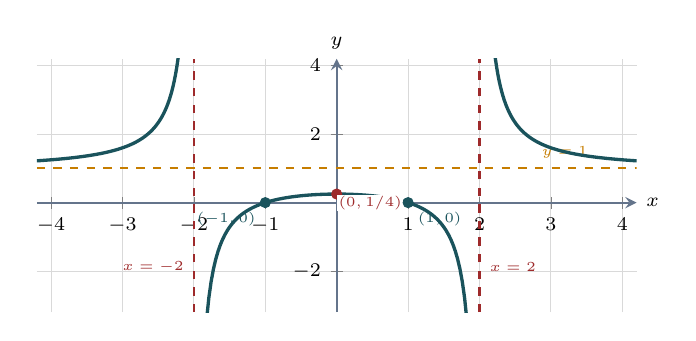
\begin{tikzpicture}
\begin{axis}[
    width=9.2cm, height=4.8cm,
    xmin=-4.2, xmax=4.2,
    ymin=-3.2, ymax=4.2,
    axis lines=middle,
    axis line style={-stealth, thick, color=slateMuted},
    xlabel={$x$}, ylabel={$y$},
    grid=both,
    grid style={line width=.2pt, draw=gray!20},
    major grid style={line width=.4pt, draw=gray!30},
    tick label style={font=\scriptsize},
    xlabel style={at={(ticklabel* cs:1)},anchor=west, font=\scriptsize},
    ylabel style={at={(ticklabel* cs:1)},anchor=south, font=\scriptsize},
    restrict y to domain=-5.5:5.5,
    samples=120
]
    \draw[dashed, thick, ponchoRed] (-2, -3.2) -- (-2, 4.2) node[pos=0.18, left, font=\tiny\bfseries] {$x=-2$};
    \draw[dashed, thick, ponchoRed] (2, -3.2) -- (2, 4.2) node[pos=0.18, right, font=\tiny\bfseries] {$x=2$};
    \draw[dashed, thick, incaGold] (-4.2, 1) -- (4.2, 1) node[pos=0.88, above, font=\tiny\bfseries] {$y=1$};

    \addplot[domain=-4.2:-2.08, color=amarunTeal, very thick] {(x^2 - 1)/(x^2 - 4)};
    \addplot[domain=-1.92:1.92, color=amarunTeal, very thick] {(x^2 - 1)/(x^2 - 4)};
    \addplot[domain=2.08:4.2, color=amarunTeal, very thick] {(x^2 - 1)/(x^2 - 4)};

    \filldraw[ponchoRed] (0, 0.25) circle (1.8pt) node[below right, font=\tiny, fill=white, inner sep=0.5pt] {$(0, 1/4)$};
    \filldraw[amarunTeal] (-1, 0) circle (1.8pt) node[below left, font=\tiny] {$(-1, 0)$};
    \filldraw[amarunTeal] (1, 0) circle (1.8pt) node[below right, font=\tiny] {$(1, 0)$};
\end{axis}
\end{tikzpicture}\\[-3pt]
{\scriptsize\color{slateMuted}\textbf{Gráfico 1:} Curva racional $f(x) = \frac{x^2 - 1}{x^2 - 4}$ con 3 ramas, asíntotas $x = \pm 2, y = 1$ y hueco en $\left(\frac{1}{4}, 1\right]$.}
\end{center}

\begin{resultadobox}
\textbf{Resultado Final:} $\operatorname{Dom}(f) = \mathbb{R}\setminus\{-2, 2\}$, asíntotas $x = \pm 2$, $y = 1$, y $\mathbf{\operatorname{Ran}(f) = \left(-\infty, \frac{1}{4}\right] \cup (1, +\infty)}$.
\end{resultadobox}
\end{solucionbox}

\newpage

% =========================================================================
% EJERCICIO 05: RACIONAL CON ASÍNTOTA OBLICUA Y GRÁFICO 2
% =========================================================================
\ejerciciotitle{Ejercicio Jh 05}{Racional Impar y Asíntota Oblicua por División}{Quiz 4 $\cdot$ Pág. 2}

\begin{enunciadobox}
\textbf{\color{amarunTeal}ENUNCIADO:} Halle las asíntotas completas (incluyendo oblicua), simetría y cortes de la función racional, y elabore su gráfico analítico:
\[ f(x) = \frac{x^3 - 4x}{x^2 - 1} \]
\end{enunciadobox}

\begin{solucionbox}
\textbf{\color{ponchoRed}SOLUCIÓN PASO A PASO:}
\begin{enumerate}
    \item \textbf{Dominio y Simetría:} $x^2 - 1 = 0 \implies \mathbf{\operatorname{Dom}(f) = \mathbb{R} \setminus \{-1, 1\}}$.
    $f(-x) = \frac{-x^3 + 4x}{x^2 - 1} = -f(x) \implies \textbf{Función Impar}$ (simétrica al origen).
    \item \textbf{Cortes Axiales:} $x(x - 2)(x + 2) = 0 \implies \mathbf{(0, 0)}$, $\mathbf{(-2, 0)}$ y $\mathbf{(2, 0)}$.
    \item \textbf{Asíntotas:} Verticales en $\mathbf{x = \pm 1}$. Por división polinomial:
    $\frac{x^3 - 4x}{x^2 - 1} = x - \frac{3x}{x^2 - 1} \implies \text{Asíntota Oblicua: } \mathbf{y = x}$.
    \item \textbf{Rango:} Cubre todos los reales $\implies \mathbf{\operatorname{Ran}(f) = \mathbb{R}}$.
\end{enumerate}

\begin{center}
% --- GRÁFICO 2: VECTORIAL PGFPLOTS ---
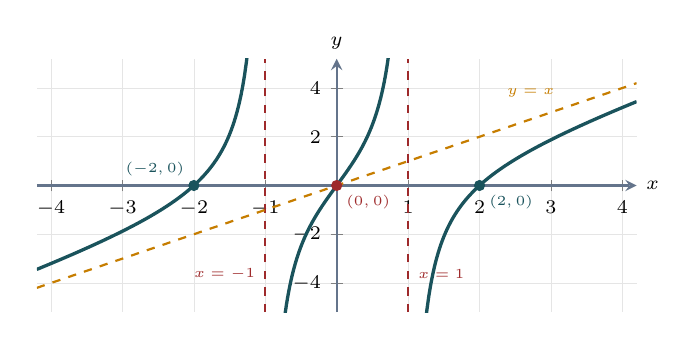
\begin{tikzpicture}
\begin{axis}[
    width=9.2cm, height=4.8cm,
    xmin=-4.2, xmax=4.2,
    ymin=-5.2, ymax=5.2,
    axis lines=middle,
    axis line style={-stealth, thick, color=slateMuted},
    xlabel={$x$}, ylabel={$y$},
    grid=both,
    grid style={line width=.2pt, draw=gray!20},
    tick label style={font=\scriptsize},
    xlabel style={at={(ticklabel* cs:1)},anchor=west, font=\scriptsize},
    ylabel style={at={(ticklabel* cs:1)},anchor=south, font=\scriptsize},
    restrict y to domain=-7:7,
    samples=120
]
    \draw[dashed, thick, ponchoRed] (-1, -5.2) -- (-1, 5.2) node[pos=0.15, left, font=\tiny\bfseries] {$x=-1$};
    \draw[dashed, thick, ponchoRed] (1, -5.2) -- (1, 5.2) node[pos=0.15, right, font=\tiny\bfseries] {$x=1$};
    \draw[dashed, thick, incaGold] (-4.2, -4.2) -- (4.2, 4.2) node[pos=0.88, above left, font=\tiny\bfseries] {$y=x$};

    \addplot[domain=-4.2:-1.08, color=amarunTeal, very thick] {(x^3 - 4*x)/(x^2 - 1)};
    \addplot[domain=-0.92:0.92, color=amarunTeal, very thick] {(x^3 - 4*x)/(x^2 - 1)};
    \addplot[domain=1.08:4.2, color=amarunTeal, very thick] {(x^3 - 4*x)/(x^2 - 1)};

    \filldraw[ponchoRed] (0, 0) circle (1.8pt) node[below right, font=\tiny] {$(0, 0)$};
    \filldraw[amarunTeal] (-2, 0) circle (1.8pt) node[above left, font=\tiny] {$(-2, 0)$};
    \filldraw[amarunTeal] (2, 0) circle (1.8pt) node[below right, font=\tiny] {$(2, 0)$};
\end{axis}
\end{tikzpicture}\\[-3pt]
{\scriptsize\color{slateMuted}\textbf{Gráfico 2:} Función impar $f(x) = \frac{x^3 - 4x}{x^2 - 1}$ con asíntotas $x = \pm 1$ y oblicua $y = x$.}
\end{center}

\begin{resultadobox}
\textbf{Resultado Final:} Función impar, asíntotas $x = \pm 1$, asíntota oblicua $y = x$, cortes en $0, \pm 2$ y $\mathbf{\operatorname{Ran}(f) = \mathbb{R}}$.
\end{resultadobox}
\end{solucionbox}

% =========================================================================
% EJERCICIO 06: RACIONAL CON MÍNIMO Y RANGO HUECO
% =========================================================================
\ejerciciotitle{Ejercicio Jh 06}{Racional Par con Rango Acotado por Extremo}{Quiz 4 $\cdot$ Pág. 3}

\begin{enunciadobox}
\textbf{\color{amarunTeal}ENUNCIADO:} Deduzca algebraicamente el rango y justifique formalmente el intervalo excluido de:
\[ f(x) = \frac{x^2 - 9}{x^2 - 1} \]
\end{enunciadobox}

\begin{solucionbox}
\textbf{\color{ponchoRed}SOLUCIÓN PASO A PASO:}
\begin{enumerate}
    \item \textbf{Dominio y Simetría:} $\operatorname{Dom}(f) = \mathbb{R} \setminus \{-1, 1\}$. Paridad: $f(-x) = f(x)$ (\textbf{Función Par}).
    \item \textbf{Cortes y Asíntotas:} Corte $Y$: $f(0) = \frac{-9}{-1} = 9 \implies \mathbf{(0, 9)}$ (mínimo local). Cortes $X$: $\mathbf{(\pm 3, 0)}$.
    Asíntotas verticales en $x = \pm 1$; Horizontal en $\mathbf{y = 1}$.
    \item \textbf{Deducción del Rango:} $y = \frac{x^2 - 9}{x^2 - 1} \implies x^2(y - 1) = y - 9 \implies x^2 = \frac{y - 9}{y - 1} \ge 0$.
    Puntos de prueba: $y = 1$ (abierto) y $y = 9$ (cerrado). El signo es positivo en $(-\infty, 1) \cup [9, +\infty)$.
\end{enumerate}
\begin{resultadobox}
\textbf{Resultado Final:} $\mathbf{\operatorname{Ran}(f) = (-\infty, 1) \cup [9, +\infty)}$. El intervalo $[1, 9)$ no tiene preimagen real.
\end{resultadobox}
\end{solucionbox}

\newpage

% =========================================================================
% EJERCICIO 07: RADICAL
% =========================================================================
\ejerciciotitle{Ejercicio Jh 07}{Función Radical con Dominio Discontinuo}{Quiz 4 $\cdot$ Pág. 3}

\begin{enunciadobox}
\textbf{\color{amarunTeal}ENUNCIADO:} Halle el dominio maximal y determine el rango de la función radical:
\[ f(x) = \sqrt{\frac{x^2 - 1}{x^2 - 4}} \]
\end{enunciadobox}

\begin{solucionbox}
\textbf{\color{ponchoRed}SOLUCIÓN PASO A PASO:}
\begin{enumerate}
    \item \textbf{Dominio Maximal:} Requiere $\frac{x^2 - 1}{x^2 - 4} \ge 0$ con $x \ne \pm 2$. Puntos críticos: $x = \pm 1, \pm 2$.
    Por tabla de signos: $\mathbf{\operatorname{Dom}(f) = (-\infty, -2) \cup [-1, 1] \cup (2, +\infty)}$.
    \item \textbf{Cortes Axiales:} Corte $Y$: $f(0) = \sqrt{\frac{1}{4}} = \frac{1}{2} \implies \mathbf{\left(0, \frac{1}{2}\right)}$. Cortes $X$: $\mathbf{(\pm 1, 0)}$.
    \item \textbf{Rango:} Como $f(x) = \sqrt{g(x)}$ con $\operatorname{Ran}(g) = (-\infty, 1/4] \cup (1, \infty)$ y la raíz exige valores $\ge 0$:
    $\operatorname{Ran}(f) = \left[0, \sqrt{1/4}\right] \cup (\sqrt{1}, +\infty) = \mathbf{\left[0, \frac{1}{2}\right] \cup (1, +\infty)}$.
\end{enumerate}
\begin{resultadobox}
\textbf{Resultado Final:} $\operatorname{Dom}(f) = (-\infty, -2) \cup [-1, 1] \cup (2, +\infty)$ y $\mathbf{\operatorname{Ran}(f) = \left[0, \frac{1}{2}\right] \cup (1, +\infty)}$.
\end{resultadobox}
\end{solucionbox}

% =========================================================================
% EJERCICIO 08: INVERSA FORMAL CON GRÁFICO 3
% =========================================================================
\ejerciciotitle{Ejercicio Jh 08}{Biyectividad, Función Inversa y Simetría}{Guía 2.6 $\cdot$ Pág. 3}

\begin{enunciadobox}
\textbf{\color{amarunTeal}ENUNCIADO:} Sea la función cuadrática con dominio restringido:
\[ f: [0, +\infty) \longrightarrow [1, +\infty), \qquad f(x) = x^2 + 1 \]
Demuestre formalmente que es inyectiva y sobreyectiva (biyectiva), deduzca la fórmula de $f^{-1}(x)$ y represente gráficamente ambas curvas con el eje de simetría $y = x$.
\end{enunciadobox}

\begin{solucionbox}
\textbf{\color{ponchoRed}SOLUCIÓN PASO A PASO:}
\begin{enumerate}
    \item \textbf{Demostración de Inyectividad:} Sean $x_1, x_2 \ge 0$ tales que $f(x_1) = f(x_2)$:
    \[ x_1^2 + 1 = x_2^2 + 1 \implies x_1^2 = x_2^2 \implies \sqrt{x_1^2} = \sqrt{x_2^2} \implies |x_1| = |x_2| \]
    Al ser $x_1, x_2 \ge 0$, se tiene $x_1 = x_2 \implies \mathbf{f \text{ es inyectiva}}$.
    \item \textbf{Demostración de Sobreyectividad:} Para todo $y \ge 1$, $y = x^2 + 1 \implies x = \sqrt{y - 1}$ (raíz positiva pues $x \ge 0$).
    Como $y \ge 1 \implies y - 1 \ge 0$, existe $x \in [0, +\infty) \implies \mathbf{f \text{ es sobreyectiva}}$.
    \item \textbf{Función Inversa:} Al ser biyectiva: $\mathbf{f^{-1}(x) = \sqrt{x - 1}}$, $\operatorname{Dom}(f^{-1}) = [1, +\infty)$, $\operatorname{Ran}(f^{-1}) = [0, +\infty)$.
\end{enumerate}

\begin{center}
% --- GRÁFICO 3: VECTORIAL PGFPLOTS ---
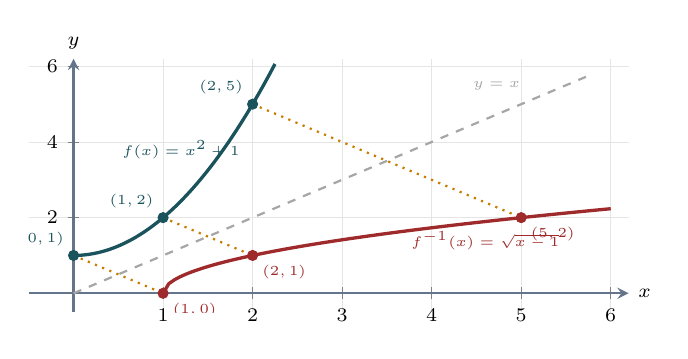
\begin{tikzpicture}
\begin{axis}[
    width=9.2cm, height=4.8cm,
    xmin=-0.5, xmax=6.2,
    ymin=-0.5, ymax=6.2,
    axis lines=middle,
    axis line style={-stealth, thick, color=slateMuted},
    xlabel={$x$}, ylabel={$y$},
    grid=both,
    grid style={line width=.2pt, draw=gray!20},
    tick label style={font=\scriptsize},
    xlabel style={at={(ticklabel* cs:1)},anchor=west, font=\scriptsize},
    ylabel style={at={(ticklabel* cs:1)},anchor=south, font=\scriptsize},
]
    \draw[dashed, thick, gray!70] (0, 0) -- (5.8, 5.8) node[pos=0.88, above left, font=\tiny\bfseries] {$y = x$};

    \addplot[domain=0:2.25, color=amarunTeal, very thick, samples=80] {x^2 + 1};
    \node[color=amarunTeal, font=\tiny\bfseries] at (axis cs:1.2, 3.8) {$f(x) = x^2 + 1$};

    \addplot[domain=1:6.0, color=ponchoRed, very thick, samples=80] {sqrt(x - 1)};
    \node[color=ponchoRed, font=\tiny\bfseries] at (axis cs:4.6, 1.4) {$f^{-1}(x) = \sqrt{x-1}$};

    \draw[dotted, thick, incaGold] (0, 1) -- (1, 0);
    \draw[dotted, thick, incaGold] (1, 2) -- (2, 1);
    \draw[dotted, thick, incaGold] (2, 5) -- (5, 2);

    \filldraw[amarunTeal] (0, 1) circle (1.8pt) node[above left, font=\tiny] {$(0, 1)$};
    \filldraw[ponchoRed] (1, 0) circle (1.8pt) node[below right, font=\tiny] {$(1, 0)$};
    \filldraw[amarunTeal] (1, 2) circle (1.8pt) node[above left, font=\tiny] {$(1, 2)$};
    \filldraw[ponchoRed] (2, 1) circle (1.8pt) node[below right, font=\tiny] {$(2, 1)$};
    \filldraw[amarunTeal] (2, 5) circle (1.8pt) node[above left, font=\tiny] {$(2, 5)$};
    \filldraw[ponchoRed] (5, 2) circle (1.8pt) node[below right, font=\tiny] {$(5, 2)$};
\end{axis}
\end{tikzpicture}\\[-3pt]
{\scriptsize\color{slateMuted}\textbf{Gráfico 3:} Simetría axial respecto a $y = x$ entre $f(x) = x^2 + 1$ y su inversa $f^{-1}(x) = \sqrt{x - 1}$.}
\end{center}

\begin{resultadobox}
\textbf{Resultado Final:} $f$ es biyectiva con $\mathbf{f^{-1}(x) = \sqrt{x - 1}}$, $\operatorname{Dom}(f^{-1}) = [1, +\infty)$ y simetría en $(x, y) \leftrightarrow (y, x)$.
\end{resultadobox}
\end{solucionbox}

\newpage

% =========================================================================
% EJERCICIO 09: TRANSFORMACIONES Y FORMA CANÓNICA
% =========================================================================
\ejerciciotitle{Ejercicio Jh 09}{Transformaciones Cuadráticas y Vértice}{Guía 2.5 $\cdot$ Pág. 3}

\begin{enunciadobox}
\textbf{\color{amarunTeal}ENUNCIADO:} A partir de la parábola estándar $f(x) = x^2$, determine la secuencia de transformaciones geométricas que producen la función:
\[ g(x) = -\frac{3}{2}(2x + 4)^2 + 5 \]
y exprésela en la forma canónica de vértice $g(x) = a(x - h)^2 + k$.
\end{enunciadobox}

\begin{solucionbox}
\textbf{\color{ponchoRed}SOLUCIÓN PASO A PASO:}
\begin{enumerate}
    \item \textbf{Factorización Canónica Rigurosa:}
    \[ g(x) = -\frac{3}{2}\left[2(x + 2)\right]^2 + 5 = -\frac{3}{2} \cdot 4(x + 2)^2 + 5 = \mathbf{-6(x + 2)^2 + 5} \implies \mathbf{V(-2, 5)} \]
    \item \textbf{Secuencia de Transformaciones:} Traslación horizontal de $2\text{ u a la izquierda } (x \to x+2)$; dilatación vertical $\times 6$; reflexión en eje $X$ (invierte $Y$); y traslación vertical de $5\text{ u hacia arriba}$.
    \item \textbf{Equivalencia Guía 2.5:} Compresión horizontal $\times \frac{1}{2}$, dilatación vertical $\times \frac{3}{2}$ y reflexión en $X$, equivalente pues $2^2 \times \frac{3}{2} = 6$.
\end{enumerate}
\begin{resultadobox}
\textbf{Resultado Final:} Forma canónica $\mathbf{g(x) = -6(x + 2)^2 + 5}$, vértice $V(-2, 5)$ y apertura hacia abajo.
\end{resultadobox}
\end{solucionbox}

% =========================================================================
% EJERCICIO 10: COMPARACIÓN DE OPERADORES CON GRÁFICO 4
% =========================================================================
\ejerciciotitle{Ejercicio Jh 10}{Operadores de Transformación Externos vs Internos}{Guía 2.5 $\cdot$ Pág. 3}

\begin{enunciadobox}
\textbf{\color{amarunTeal}ENUNCIADO:} Compare analítica y geométricamente las transformaciones de:
\[ g(x) = -2f(x - 3) + 4 \qquad \text{vs} \qquad h(x) = f(-2(x - 3)) + 4 \]
Ilustre el comportamiento de ambas transformaciones tomando como prototipo la función $f(x) = \sqrt{x}$.
\end{enunciadobox}

\begin{solucionbox}
\textbf{\color{ponchoRed}SOLUCIÓN PASO A PASO:}
\begin{enumerate}
    \item \textbf{Cuadro Comparativo de Propiedades:}
    \vspace{1pt}
    \begin{center}
    \footnotesize
    \renewcommand{\arraystretch}{0.92}
    \begin{tabularx}{\linewidth}{@{}lXX@{}}
    \toprule
    \textbf{Operación} & \textbf{Para } $g(x) = -2f(x - 3) + 4$ & \textbf{Para } $h(x) = f(-2(x - 3)) + 4$ \\
    \midrule
    \textbf{Desplazamiento $X$} & $3\text{ u a la derecha } (x \to x + 3)$ & $3\text{ u a la derecha } (x \to x + 3)$ \\
    \textbf{Factor de Escala} & \textbf{Dilatación vertical de factor 2} & \textbf{Compresión horizontal de factor } $\mathbf{\frac{1}{2}}$ \\
    \textbf{Reflexión} & \textbf{Respecto al eje $X$} (invierte alturas $Y$) & \textbf{Respecto al eje $Y$} (invierte horizontal $X$) \\
    \textbf{Desplazamiento $Y$} & $4\text{ u hacia arriba } (y \to y + 4)$ & $4\text{ u hacia arriba } (y \to y + 4)$ \\
    \midrule
    \textbf{Mapeo Coordenado} & $(x, y) \longrightarrow \mathbf{(x + 3, \; -2y + 4)}$ & $(x, y) \longrightarrow \mathbf{\left(-\frac{x}{2} + 3, \; y + 4\right)}$ \\
    \bottomrule
    \end{tabularx}
    \end{center}
    \item \textbf{Comportamiento con Prototipo $f(x) = \sqrt{x}$:} Ambas curvas comparten el vértice ancla $(3, 4)$. La función $g(x) = -2\sqrt{x-3}+4$ se proyecta hacia \textbf{abajo-derecha} ($\operatorname{Dom} = [3, \infty), \operatorname{Ran} = (-\infty, 4]$) mientras $h(x) = \sqrt{-2(x-3)}+4$ se proyecta hacia \textbf{arriba-izquierda} ($\operatorname{Dom} = (-\infty, 3], \operatorname{Ran} = [4, \infty)$).
\end{enumerate}

\begin{center}
% --- GRÁFICO 4: VECTORIAL PGFPLOTS ---
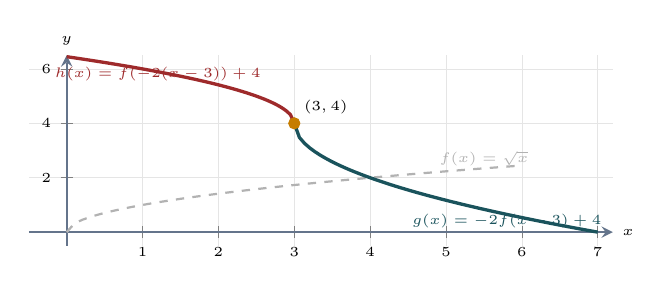
\begin{tikzpicture}
\begin{axis}[
    width=9.0cm, height=4.0cm,
    xmin=-0.5, xmax=7.2,
    ymin=-0.5, ymax=6.5,
    axis lines=middle,
    axis line style={-stealth, thick, color=slateMuted},
    xlabel={$x$}, ylabel={$y$},
    grid=both,
    grid style={line width=.2pt, draw=gray!20},
    tick label style={font=\tiny},
    xlabel style={at={(ticklabel* cs:1)},anchor=west, font=\tiny},
    ylabel style={at={(ticklabel* cs:1)},anchor=south, font=\tiny},
    unbounded coords=discard
]
    \addplot[domain=0:6, dashed, color=gray!60, thick, samples=60] {sqrt(x)};
    \node[color=gray!60, font=\tiny] at (axis cs:5.5, 2.7) {$f(x)=\sqrt{x}$};

    \addplot[domain=3:7, color=amarunTeal, very thick, samples=60] {-2*sqrt(x - 3) + 4};
    \node[color=amarunTeal, font=\tiny\bfseries] at (axis cs:5.8, 0.4) {$g(x)=-2f(x-3)+4$};

    \addplot[domain=0:3, color=ponchoRed, very thick, samples=60] {sqrt(max(0, -2*(x - 3))) + 4};
    \node[color=ponchoRed, font=\tiny\bfseries] at (axis cs:1.2, 5.8) {$h(x)=f(-2(x-3))+4$};

    \filldraw[incaGold] (3, 4) circle (2.0pt) node[above right, font=\tiny\bfseries, color=black] {$(3, 4)$};
\end{axis}
\end{tikzpicture}\\[-4pt]
{\scriptsize\color{slateMuted}\textbf{Gráfico 4:} Comparación de operadores sobre $f(x) = \sqrt{x}$ anclados en el punto $(3, 4)$.}
\end{center}

\begin{resultadobox}
\textbf{Resultado Final:} $g(x)$ opera en el codominio (afecta $Y$), mientras $h(x)$ opera en el dominio (afecta $X$).
\end{resultadobox}
\end{solucionbox}

\newpage

% =========================================================================
% PÁGINA 6: SÍNTESIS, RECONSTRUCCIÓN Y DIRECTORIO DE VIDEOS
% =========================================================================
\ejerciciotitle{Modelos Adicionales}{Reconstrucción de Ecuaciones a partir de Información Gráfica}{Guía 2.5 $\cdot$ Págs. 2 a 4}

\begin{enunciadobox}
\textbf{\color{amarunTeal}ENUNCIADO:} Halle la regla de correspondencia para las siguientes curvas estándar modificadas:
(1) Valor absoluto con vértice en $(-3, 4)$ que pasa por $(-1, 1)$; (2) Radical invertida con inicio en $(5, -2)$ que pasa por $(9, -6)$; (3) Parábola con vértice en $(4, -3)$ que pasa por $(6, 5)$.
\end{enunciadobox}

\begin{solucionbox}
\textbf{\color{ponchoRed}SOLUCIÓN PASO A PASO:}
\begin{enumerate}
    \item \textbf{Valor Absoluto $g(x) = a|x - h| + k$:}
    Vértice en $(-3, 4) \implies g(x) = a|x + 3| + 4$. Sustituyendo $(-1, 1)$:
    \[ 1 = a|-1 + 3| + 4 \implies 1 = 2a + 4 \implies 2a = -3 \implies a = -\tfrac{3}{2} \implies \mathbf{g(x) = -\frac{3}{2}|x + 3| + 4} \]
    \item \textbf{Función Radical $g(x) = -a\sqrt{x - h} + k$:}
    Inicio en $(5, -2)$ y reflejada en $X \implies g(x) = -a\sqrt{x - 5} - 2$. Sustituyendo $(9, -6)$:
    \[ -6 = -a\sqrt{9 - 5} - 2 \implies -4 = -2a \implies a = 2 \implies \mathbf{g(x) = -2\sqrt{x - 5} - 2} \]
    \item \textbf{Función Cuadrática $g(x) = a(x - h)^2 + k$:}
    Vértice en $(4, -3) \implies g(x) = a(x - 4)^2 - 3$. Sustituyendo $(6, 5)$:
    \[ 5 = a(6 - 4)^2 - 3 \implies 8 = 4a \implies a = 2 \implies \mathbf{g(x) = 2(x - 4)^2 - 3} \]
\end{enumerate}
\end{solucionbox}

\vspace{2pt}
% --- CHECKLIST DEL PROTOCOLO DE 7 PASOS ---
\begin{enunciadobox}
\textbf{\color{amarunTeal}ALGORITMO OFICIAL DE 7 PASOS PARA ASEGURAR 10/10 EN EL QUIZ 4}
\vspace{2pt}

\begin{center}
\footnotesize
\renewcommand{\arraystretch}{1.05}
\begin{tabularx}{\linewidth}{@{}clX@{}}
\toprule
\textbf{Paso} & \textbf{Etapa Evaluada} & \textbf{Requisito Indispensable para Calificación 10/10} \\
\midrule
\textbf{1} & \textbf{Dominio Maximal} & Excluir raíces negativas en índice par y división entre cero ($Q(x) \ne 0$). \\
\textbf{2} & \textbf{Cortes Axiales} & Eje $Y$: evaluar $f(0)$; Eje $X$: resolver analíticamente $f(x) = 0$. \\
\textbf{3} & \textbf{Simetría (Paridad)} & Evaluar $f(-x)$: si es $f(x)$ (Par / eje $Y$); si es $-f(x)$ (Impar / origen). \\
\textbf{4} & \textbf{Asíntotas Completas} & Verticales (polos), Horizontales ($\lim_{x \to \pm\infty}$) y Oblicuas ($y = mx+b$). \\
\textbf{5} & \textbf{Intervalos y Signos} & Tabla de factores separando $(+)$ y $(-)$ entre raíces y polos. \\
\textbf{6} & \textbf{Bosquejo Gráfico} & Trazar asíntotas punteadas, cortes y curvas asintóticas nítidas. \\
\textbf{7} & \textbf{Rango Deductivo} & Despejar $x$ en función de $y$, aplicar $x^2 \ge 0$ o inecuaciones. \\
\bottomrule
\end{tabularx}
\end{center}
\end{enunciadobox}

\vspace{2pt}
% --- DIRECTORIO DE VIDEOS MANIM 1080p60 ---
\begin{solucionbox}
\textbf{\color{amarunTeal}DIRECTORIO DE ANIMACIONES FULL HD (1080p60) DISPONIBLES}
\vspace{2pt}

\footnotesize
\renewcommand{\arraystretch}{0.92}
\begin{tabularx}{\linewidth}{@{}ccXlc@{}}
\toprule
\textbf{ID} & \textbf{Origen} & \textbf{Función / Tema Analizado} & \textbf{Archivo de Video} & \textbf{Duración} \\
\midrule
\textbf{Jh 01} & Quiz 4 & $f(x) = -\frac{1}{2}x^2 + \frac{3}{2}x + \frac{27}{8}$ (Parábola completa) & \texttt{EjercicioJh\_01.mp4} & $62\text{ s}$ \\
\textbf{Jh 02} & Quiz 4 & $f(x) = \frac{1}{2}x^3 - \frac{3}{2}x$ (Cúbica impar y simetría al origen) & \texttt{EjercicioJh\_02.mp4} & $58\text{ s}$ \\
\textbf{Jh 03} & Quiz 4 & $f(x) = \frac{1}{4}x^4 - \frac{3}{2}x^2 + \frac{5}{4}$ (Bicuadrática par) & \texttt{EjercicioJh\_03.mp4} & $60\text{ s}$ \\
\textbf{Jh 04} & Quiz 4 & $f(x) = \frac{x^2 - 1}{x^2 - 4}$ (Racional de 3 ramas con asíntotas) & \texttt{EjercicioJh\_04.mp4} & $64\text{ s}$ \\
\textbf{Jh 05} & Quiz 4 & $f(x) = \frac{x^3 - 4x}{x^2 - 1}$ (Asíntota oblicua $y = x$) & \texttt{EjercicioJh\_05.mp4} & $61\text{ s}$ \\
\textbf{Jh 06} & Quiz 4 & $f(x) = \frac{x^2 - 9}{x^2 - 1}$ (Rango con hueco por mínimo en $(0, 9)$) & \texttt{EjercicioJh\_06.mp4} & $63\text{ s}$ \\
\textbf{Jh 07} & Quiz 4 & $f(x) = \sqrt{\frac{x^2 - 1}{x^2 - 4}}$ (Radical par y dominio discontinuo) & \texttt{EjercicioJh\_07.mp4} & $62\text{ s}$ \\
\textbf{Jh 08} & Guía 2.6 & $f(x) = x^2 + 1 \implies f^{-1}(x) = \sqrt{x - 1}$ (Inversa formal) & \texttt{EjercicioJh\_08.mp4} & $61\text{ s}$ \\
\textbf{Jh 09} & Guía 2.5 & $g(x) = -\frac{3}{2}(2x + 4)^2 + 5 = -6(x + 2)^2 + 5$ & \texttt{EjercicioJh\_09.mp4} & $59\text{ s}$ \\
\textbf{Jh 10} & Guía 2.5 & $g(x) = -2f(x - 3) + 4$ vs $h(x) = f(-2(x - 3)) + 4$ & \texttt{EjercicioJh\_10.mp4} & $61\text{ s}$ \\
\bottomrule
\end{tabularx}
\end{solucionbox}

\vspace{1pt}
\begin{resultadobox}
\centering
\color{emeraldGreen}\bfseries ¡Mucho éxito en el Quiz 4, Jhoselyn! Siguiendo este esquema deductivo paso a paso asegurarás la calificación de 10/10.
\end{resultadobox}

\end{document}
